\documentclass{acmsiggraph}
\usepackage{mathptmx}
\usepackage{graphicx}

\usepackage{parskip}

%%% short abstract
% By treating an image as a two-dimensional histogram, density-field
% data sets such as those created by chaotic maps can be visualized
% much more effectively and at interactive speeds.

\onlineid{poster\_0071}

\acmformat{print}

\title{Mapping Chaos (poster\_0071)}
\author{
  David Trowbridge\thanks{e-mail: trowbrds@cs.colorado.edu}
\and
  Micah Dowty\thanks{e-mail: micah@navi.cx}
}

\keywords{iterated function systems, chaotic maps, high dynamic range, animation}

\begin{document}

\maketitle

\section{Introduction}
\copyrightspace
Iterated Function Systems are a celebrated class of dynamical systems in the
computer graphics world. By defining a constrictive set of functions and
recursing, beautiful fractal images can be created. Classically, these
systems use a set of affine transformations, such as Sierpinski's Gasket.
The addition of nonlinear transformations creates the popular ``flame''
fractal. A subclass of these are chaotic maps. Whereas traditional iterated
function systems use a set equation to create a tree structure, chaotic maps
iterate a single equation. This creates a single reproducable orbit through
the space occupied by the attractor. As the point jumps around it exposes
itself onto the image region, leaving a characteristic picture of the map.

insert more relavent, poignant, short paragraph here

\section{Exposition}
Generally the literature discussing chaotic maps and other systems which
produce density fields is full of black and white images, created where
each pixel is darkened as the point moves around the image region. This
technique is often sufficient for analyzing the structure of a map but
does not provide a sound basis for the use of the map as an artistic
entity. The structure of the attractor is only minimally visible using
such techniques, because a long iteration run will quickly result in a
completely black image.

Instead, our technique treats the entire image region as a two dimensional histogram.
Unlike previous techniques, where each $x_n$ and $y_n$ plotted by darkening a
a pixel directly, this histogram technique maintains total image intensity as
more iterations are performed. As more samples accumulate in the histogram,
the image simply gets more detailed. Instead of an image containing only a
few thousand iterations of the map, millions or billions of points can be
plotted with no loss of detail.

\begin{figure}[ht]
\centering
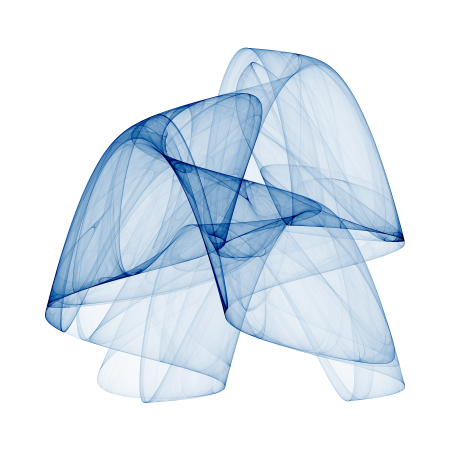
\includegraphics[width=2.5in]{1.png}
\caption{A complex attractor rendered as a two-dimensional histogram.
Fine details are made easily visible by color and shading}
\end{figure}

Like other rendering techniques that progressively refine an image, this
histogram method performes particularly well in interactive applications.
Our software for interactively browsing parameter space runs iterations
for each frame only until a predetermined amount of time has elapsed,
displaying a low quality but complete image nearly instantaneously.
Instead of waiting for a preset number of iterations to complete, the user
can zoom through parameter space quickly, viewing only what the CPU has time
to render. As soon as the user stops changing parameters, the image quality
will begin to improve.

Because a particular histogram bucket may contain tens of thousands of hits,
high-dynamic-range image processing techniques can be applied. This includes
gamma correction, exposure control, and color interpolation at the histogram's
full precision. By clamping each color component as late as possible in the
rendering process, the color can provide a visual hint at the higher
dynamic range of the image.

A histogram of infinitely small points can not be antialiased, but aliasing
artifacts can be reduced by oversampling- using multiple histogram buckets
per pixel.


\section{Conclusion}

\end{document}
